As hard radiation cannot be stopped by a moderate lead thickness, cosmic vetos are employed which consist of two complementary detectors in coincidence that provide a signal for events simultaneously detected in both of them. As shown in Figure \ref{fig:VetoAndPrototype}, the two complementary detectors are placed one above and the other below the TRITIUM detector. The distance between both detectors is $34.2~\cm$, just enough to enclose the TRITIUM IFIC prototype.

\begin{figure}[h]
\centering
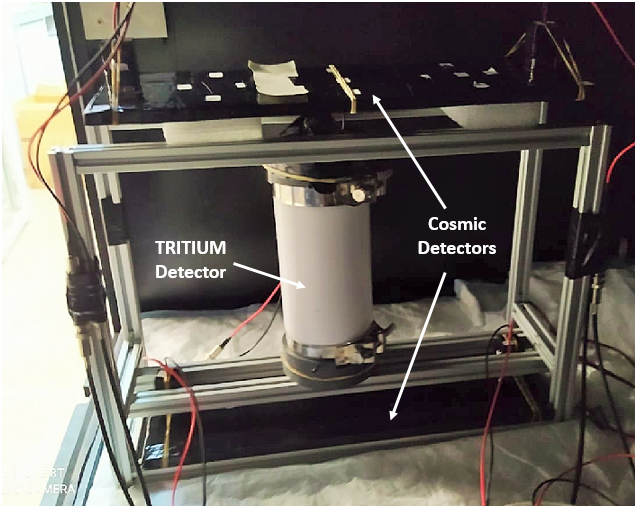
\includegraphics[scale=0.5]{3DesignPrinciples/34BackgroundRejectionSystem/Vetos_y_prototipo.png}
\caption{Cosmic veto and Tritium-IFIC-2 prototype inside the aluminium mechanical structure developed at IFIC.\label{fig:VetoAndPrototype}}
\end{figure}

A hard cosmic event crossing simultaneously both cosmic detectors is sketched in figure \ref{subfig:RealHardCosmicEvent}. Each cosmic detector has two photosensors, so the electronic configuration given in Figure \ref{subfig:ElectronicConfiguraiton4PMT} is used to make time coincidence. The TRITIUM detector is read out in anti-coincidence with the cosmic veto to reject the hard cosmic events from the tritium measurements. The expected hard cosmic rate at sea level for muons is $7\times 10^{-3}~\cm^{-2}\second^{-1}\steradian^{-1}$ \cite{PDG, HardCosmicMuonRate}, as shown in Figure \ref{fig:HardCoscmicRate}. As time coincidences are triggered by logic gates of about $10~\nano\second$, the probability of recording two different hard cosmic events in coincidence is negligible.

\begin{figure}[h]
\centering
    \begin{subfigure}[b]{0.45\textwidth}
    \centering
    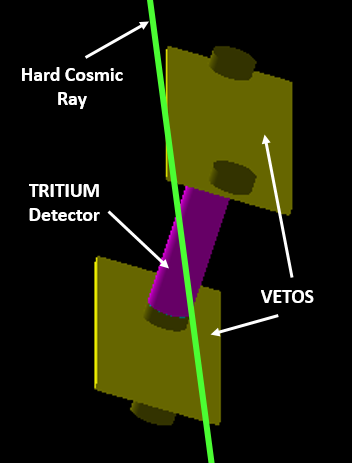
\includegraphics[width=\textwidth]{3DesignPrinciples/34BackgroundRejectionSystem/Real_Event.png}  
    \caption{\label{subfig:RealHardCosmicEvent}}
    \end{subfigure}
    \hfill
    \begin{subfigure}[b]{0.45\textwidth}
    \centering
    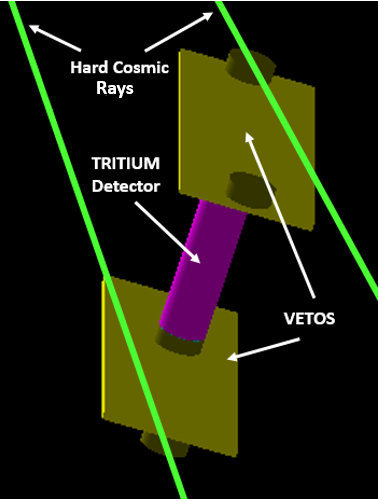
\includegraphics[width=\textwidth]{3DesignPrinciples/34BackgroundRejectionSystem/Fake_Event.png}  
    \caption{\label{subfig:FakeHardCosmicEvent}}
    \end{subfigure}
   \caption{Hard cosmic events detected with the cosmic veto of TRITIUM: a) Real coincidence event. b) Random coincidence event.}
 \label{fig:HardCosmicEventsSimulation}
\end{figure}

\begin{figure}[h]
\centering
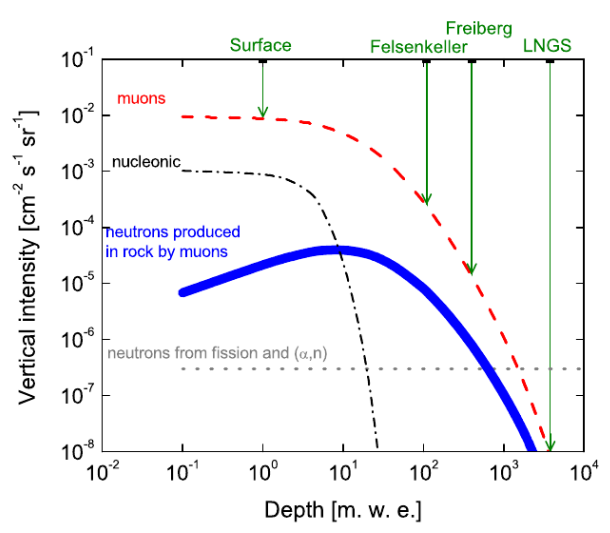
\includegraphics[scale=0.6]{3DesignPrinciples/34BackgroundRejectionSystem/HardCosmicRate.png}
\caption{Hard cosmic muon rate at different depths \cite{HardCosmicMuonRatePlot}.\label{fig:HardCoscmicRate}}
\end{figure}

The vetos are made of plastic scintillator from Epic-Crystal \cite{ScintillatorVeto} which characteristics are given in Table \ref{tab:ParametersScintillatorVeto} and its energy emission spectrum is displayed in Figure \ref{fig:EmissionEnergySpectrumVeto}. The energy spectrum has a peak very close to that of the scintillating fibres used, so the same photosensors are used for their read out. The dimensions of the scintillator plates are $45 \times 17 \times 1~\cm^3$. They are wrapped by three different layers, PTFE sheet, aluminium leaf and black tape, as shown in Figure \ref{fig:LayersVeto}. These layers prevent external photons from reaching the plastic scintillator and photons generated by the scintillator from escaping before reaching the photosensor. Two $2.5\times 2.5 ~\cm^2$ windows are made on the wrapping for coupling the photosensors.

\begin{table}[htbp]
\centering{}%
\begin{tabular}{lc}
\toprule 
Characteristic & Value \tabularnewline
\midrule
\midrule 
Base material & Polystyrene \tabularnewline
Growth method & Polymeric \tabularnewline
Density ($\gram/\cm^3$)& 1.05 \tabularnewline
Refractive index & 1.58 \tabularnewline
Soften temperature ($\celsius$) & 75-80 \tabularnewline
Light output (anthracene) & 50-60\% \tabularnewline
H/C ratio & 1.1 \tabularnewline
Emission peak (nm) & 415 (blue) \tabularnewline
Decay Time (ns) & 2.4 \tabularnewline
Hygroscopic & No \tabularnewline
\bottomrule
\end{tabular}
\caption{Characteristics of the plastic scintillator from Epic-Crystals~\cite{ScintillatorVeto}.}
\label{tab:ParametersScintillatorVeto}
\end{table}

\begin{figure}[]
\centering
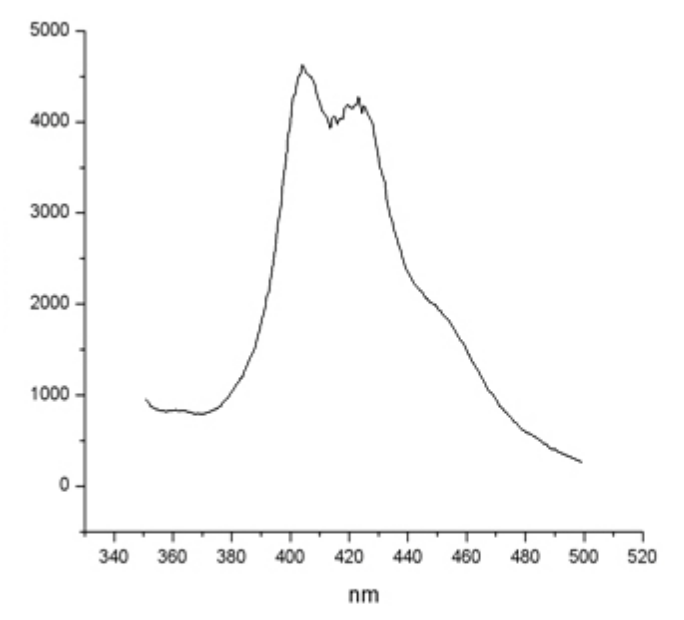
\includegraphics[scale=0.35]{3DesignPrinciples/34BackgroundRejectionSystem/EmissionEnergySpectrumVetos.png}
\caption{Emission spectrum of the plastic scintillator from \newline Epic-Crystals\label{fig:EmissionEnergySpectrumVeto}~\cite{ScintillatorVeto}.}
\end{figure}

\begin{figure}[h]
\centering
    \begin{subfigure}[b]{0.25\textwidth}
    \centering
    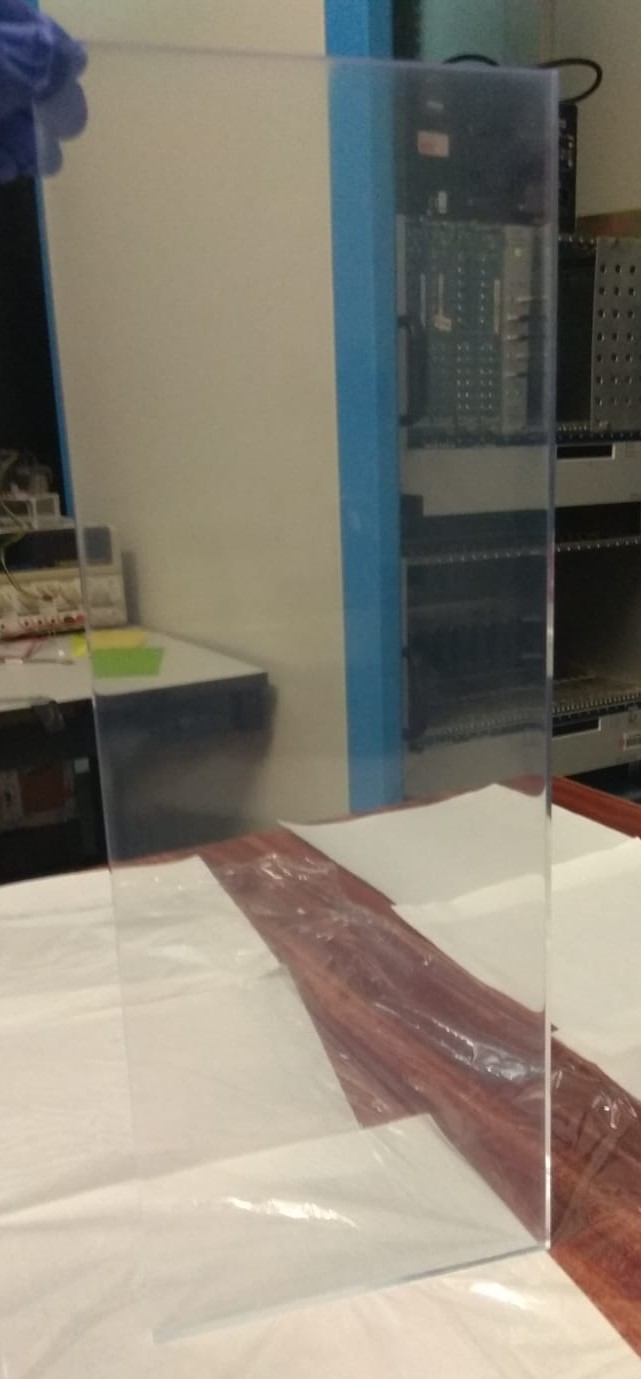
\includegraphics[width=\textwidth]{3DesignPrinciples/34BackgroundRejectionSystem/NoCoating.jpeg}  
    \caption{\label{subfig:PlasticScintillatorNoCoating}}
    \end{subfigure}
    \hfill
    \begin{subfigure}[b]{0.25\textwidth}
    \centering
    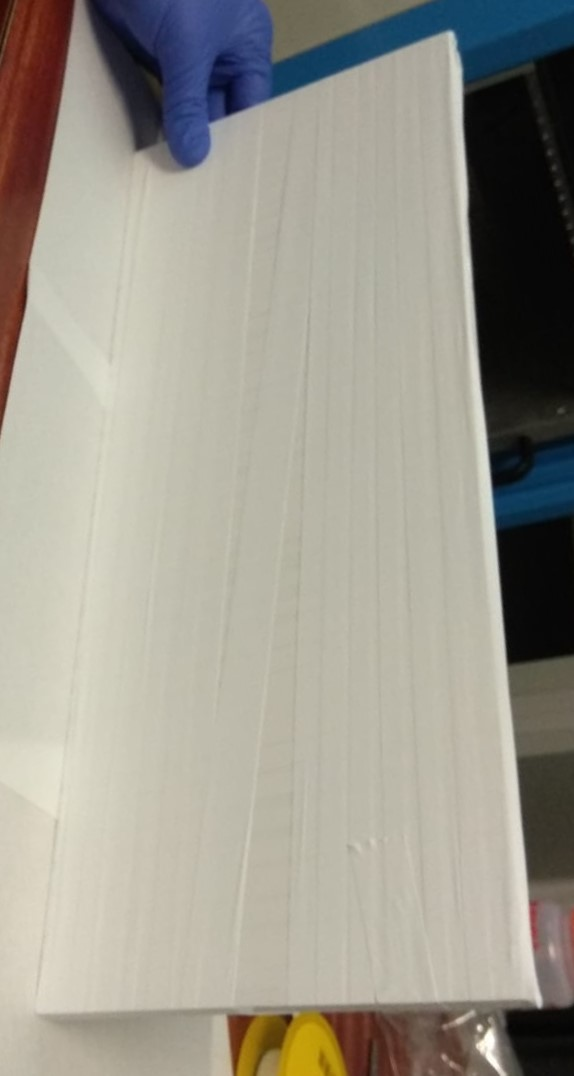
\includegraphics[width=\textwidth]{3DesignPrinciples/34BackgroundRejectionSystem/TeflonCoating.jpeg}  
    \caption{\label{subfig:PlasticScintillatorTeflon}}
    \end{subfigure}
    \newline
    \hfill
    \begin{subfigure}[b]{0.25\textwidth}
    \centering
    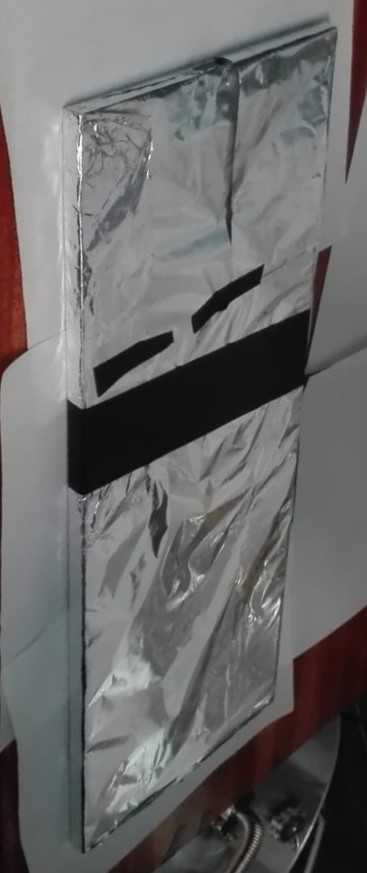
\includegraphics[width=\textwidth]{3DesignPrinciples/34BackgroundRejectionSystem/AluminiumCoating.jpeg}  
    \caption{\label{subfig:PlasticScintillatorAluminium}}
    \end{subfigure}
    \hfill
    \begin{subfigure}[b]{0.25\textwidth}
    \centering
    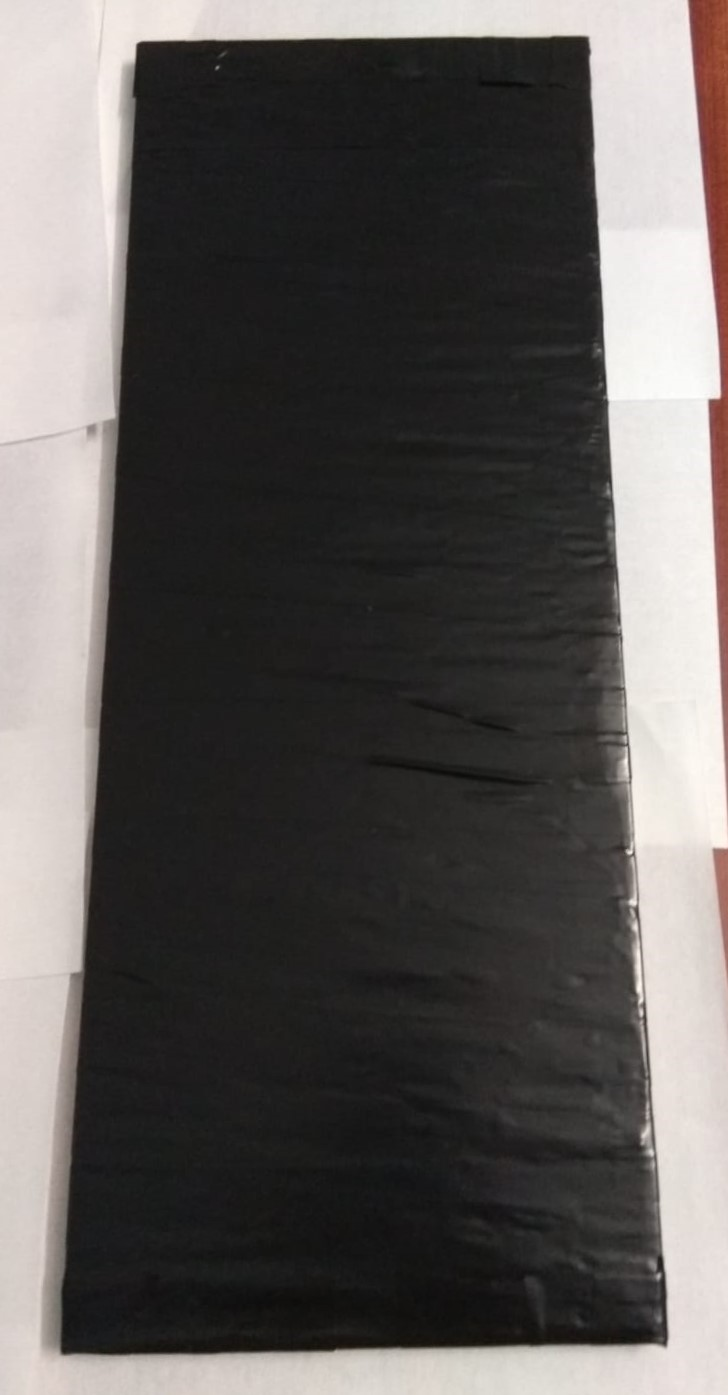
\includegraphics[width=\textwidth]{3DesignPrinciples/34BackgroundRejectionSystem/BlackTapeCoating.jpeg}  
    \caption{\label{subfig:PlasticScintillatorBlackTape}}
    \end{subfigure}
 \caption{Different layers used to wrap the cosmic veto detectors. a) Scintillator without wrapping. b) PTFE wrapping. c) Aluminium wrapping. c) d) Black tape wrapping.}
 \label{fig:LayersVeto}
\end{figure}

The solid angle subtended by each veto plate on the other is $\omega=0.5434~\steradian$ and the area is $765~\cm^2$. Considering the expected hard cosmic rate of $7 \times 10^{-3}~\cm^{-2}\second^{-1}\steradian^{-1}$ at sea level the expected hard cosmic ray rate is $2.909~\Hz$, which is used in section \ref{sec:TritiumActiveVeto} to determine the efficiency of the veto.